\documentclass{report}

\usepackage{../../../../../../LaTeX/marzstyle}

\runningheads{Computervision}{Assignment 01$_2$}

\setcounter{chapter}{1}


\begin{document}

	\section{Gradient Descent}
	\startsection
		\renewcommand{\thesubsection}{\thesection.\alph{subsection}}
		\subsection{No Regularization Gradient Descent}
		\startsubsection
			When using the Gradient Descent Algorithm with \textbf{no} \textit{Ragularization Term} ($\lambda = 0$) we get the output (\ref{fig:GD_NR}). The \textit{Loss Data Term} is therefore very low with $0.00002$ which is expected because the only thing the algorithm is trying to do is to reverse the previous blurring step. Therefore an image is created which will reproduce the blurred image when the blurring step is applied. On the other hand we get a huge squared distance difference between the deblurred and the original image with 8.21802. This is because the image contains many artifacts and the previous white parts are now in a gray shade. The artifacts (rastering of the whole image) can be traced back to the used kernel. Additionally what is noticable is that the top right and bottom left corner were unaffected because the derivative for both these cases are 0 due to the used kernel and therefore the algorithm cannot adjust those values correctly, because there is too less information in order to do that. This inaccuracy also has an effect on the adjacent pixels because the algorithm tries to create an image which will produce the same result when the blurring is repeated.
		\closesection
		\subsection{Impact of the $\lambda$ value for Gaussian Prior and Anisotropic Total Variation}
		\startsubsection
			\subsubsection{Gaussian Prior Regularization Term}
			\startsubsection
				When using the \textit{Gaussian Prior Regularization Term} the artifacts that were present without any regularization term are less pronounced and the shapes do have a more uniform color (the gradients between each pixel within a shape are lessened). Because of the introduction of a regularization term the \textit{Loss Data Term} value is increasing proportionally witht the $\lambda$ value. The best approximation of the deblurred image is reached with a $\lambda$ of 0.001 (\ref{fig:GD_GP002}). With 1,38597 this difference is still pretty high and the range of the regularization term's weight should not be too high because otherwise it will worsen the deblurring of the image. \\
				As the outputs of the algorithm (\ref{fig:GD_GP001} to \ref{fig:GD_GP1}) show, the regularization term is reducing the gradient of adjacent pixels, such that the pixels which are of approximately the same color are now more uniform. But when the $\lambda$ is too high the effect of the deblurring is reversed and the initial blurred image can be identified in the deblurred image.
			\closesection
			\subsubsection{Anisotropic Total Variation Regularization Term}
			\startsubsection
				Using the \textit{Anisotropic Total Variation Regularization Term} produces the best result for the Gradient Descent method. Again it is uniforming the values of the pixels that are approximately the same, by lessening the gradient between them. For a $\lambda = 0.0075$ (\ref{fig:GD_ATV0075}) the difference to the original image is only 0.09336. Also the Loss Data Term is very small with 0.02146. Also a $\lambda$ value of $0.01$ still produces a very good deblurring result. \\
				A higher $\lambda$ on the other hand will quickly lead to worse results in which a noise is introduced, "ruining" the previous steps in order to deblur the image. Also the \textit{Loss Data Term} is "exploding" with a value of 3.24555. Therefore a correct $\lambda$ value is of highest priority for this approach.
			\closesection
		\closesection
		
		\newpage
		\subsection*{Algorithm Output for Gradient Descent}
		\startsubsection
			The following section contains the outputs of the \textit{Gradient Descent Algorithm} from the Jupyter Notebook, which were referenced in previous sections.
			\subsubsection*{No Regularization}
			\begin{figure}[H] \renewcommand\thesubfigure{GD.NR}
				\centering
				\begin{subfigure}[b]{0.7\textwidth}
					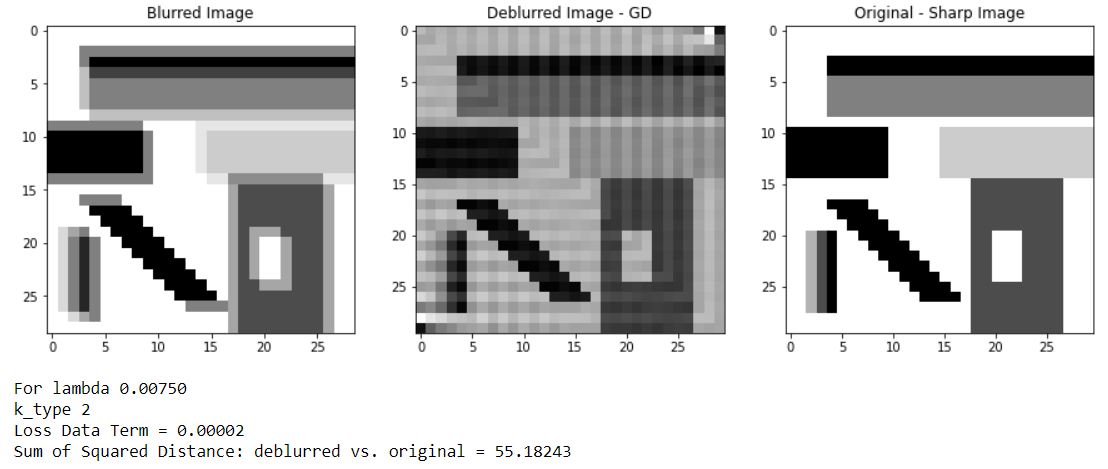
\includegraphics[scale=0.5]{GD_no_reg.png}
					\caption{Gradient Descent - \textit{No Regularization}}
					\label{fig:GD_NR}
				\end{subfigure}
			\end{figure}
			\subsubsection*{Gaussian Prior}
			\begin{figure}[H] \renewcommand\thesubfigure{GD.GP.\arabic{subfigure}}
				\centering
				\begin{subfigure}[b]{0.45\textwidth}
					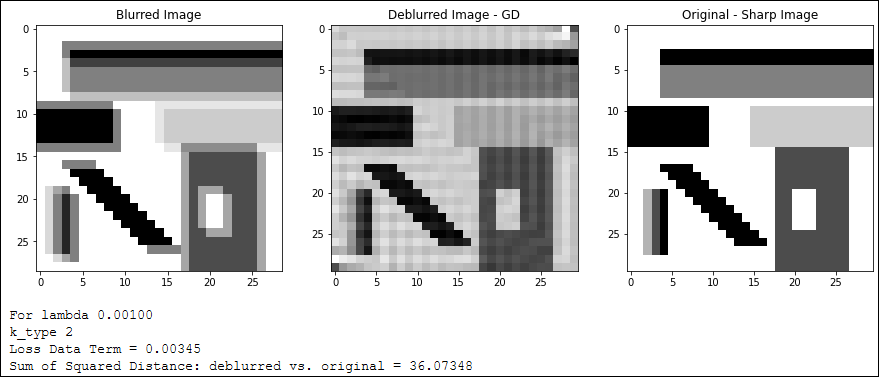
\includegraphics[scale=0.31]{GD_GP_0010.png}
					\caption{GD - \textit{Gaussian Prior}, $\lambda = 0.001$}
					\label{fig:GD_GP001}
				\end{subfigure}
				\begin{subfigure}[b]{0.45\textwidth}
					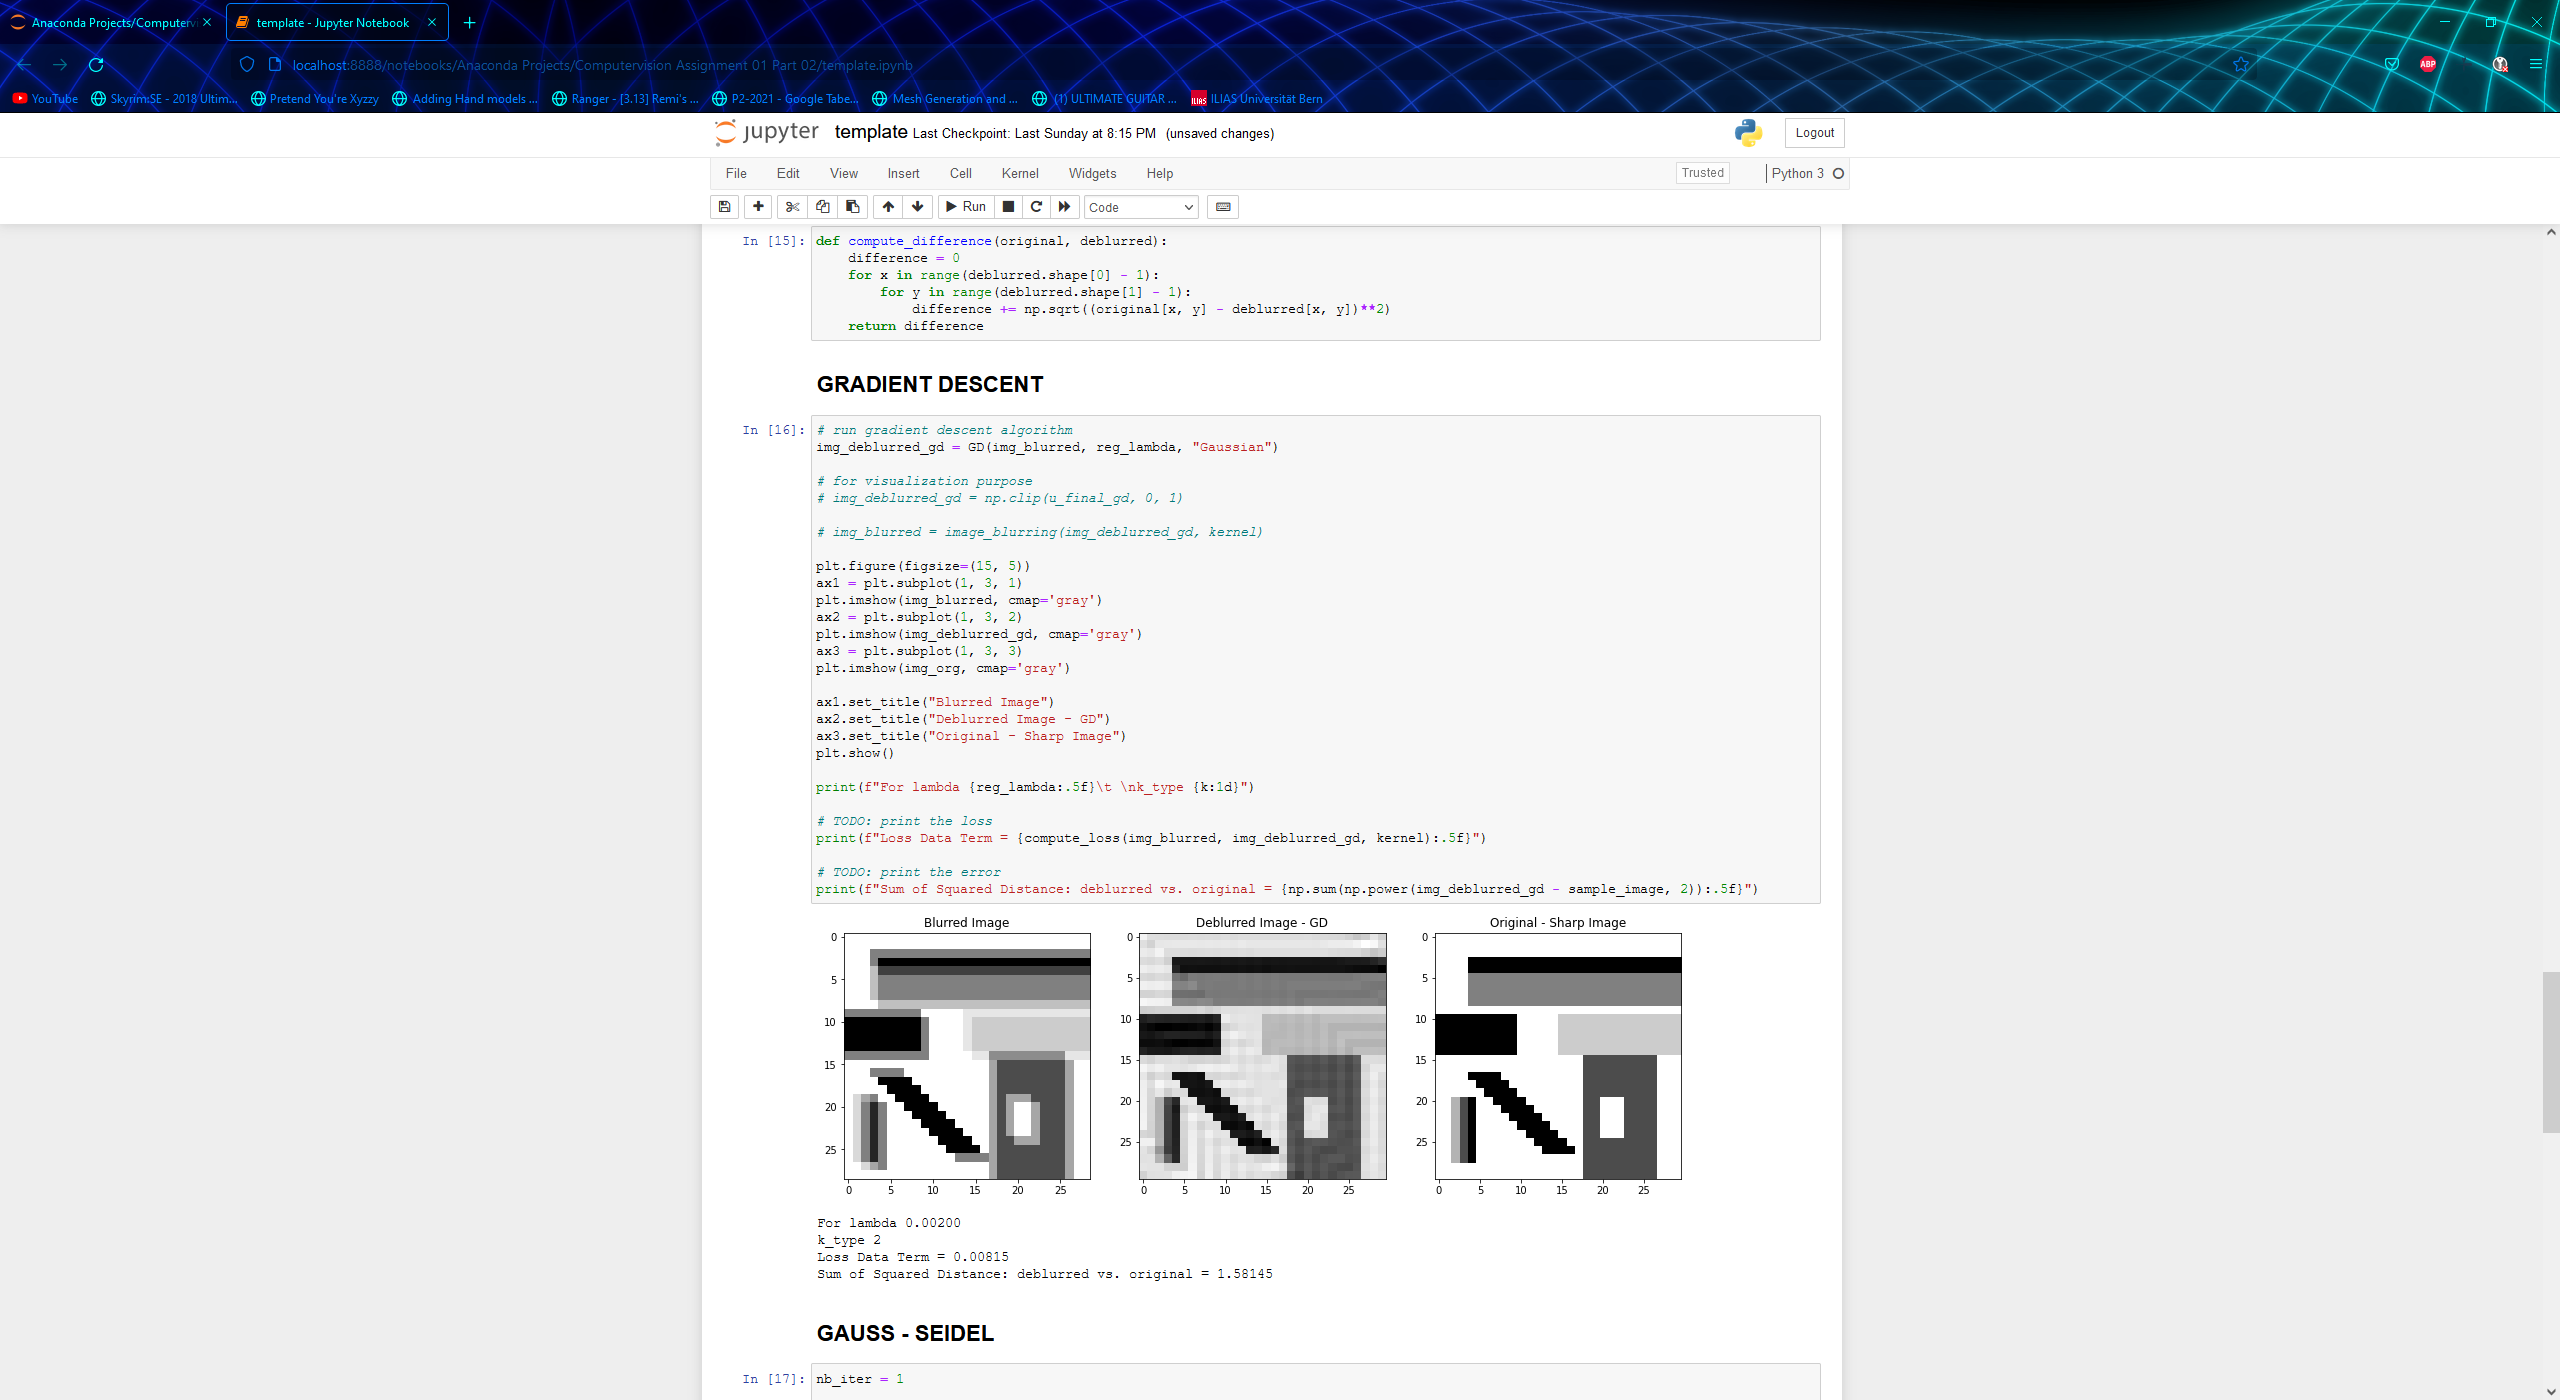
\includegraphics[scale=0.31]{GD_GP_0020.png}
					\caption{GD - \textit{Gaussian Prior}, $\lambda = 0.002$}
					\label{fig:GD_GP002}
				\end{subfigure}
				\\
				\centering
				\begin{subfigure}[b]{0.45\textwidth}
					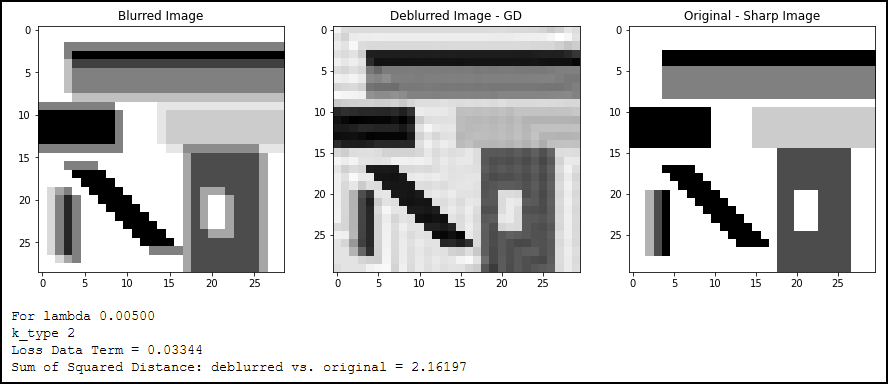
\includegraphics[scale=0.31]{GD_GP_0050.png}
					\caption{GD - \textit{Gaussian Prior}, $\lambda = 0.005$}
					\label{fig:GD_GP005}
				\end{subfigure}
				\begin{subfigure}[b]{0.45\textwidth}
					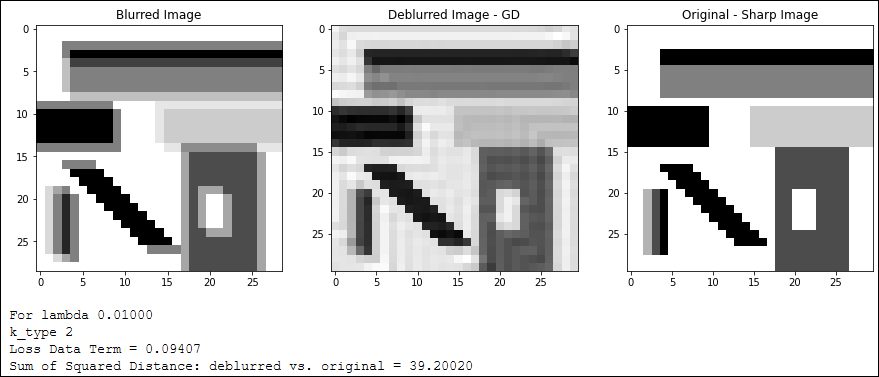
\includegraphics[scale=0.31]{GD_GP_0100.png}
					\caption{GD - \textit{Gaussian Prior}, $\lambda = 0.01$}
					\label{fig:GD_GP01}
				\end{subfigure}
				\\
				\centering
				\begin{subfigure}[b]{0.45\textwidth}
					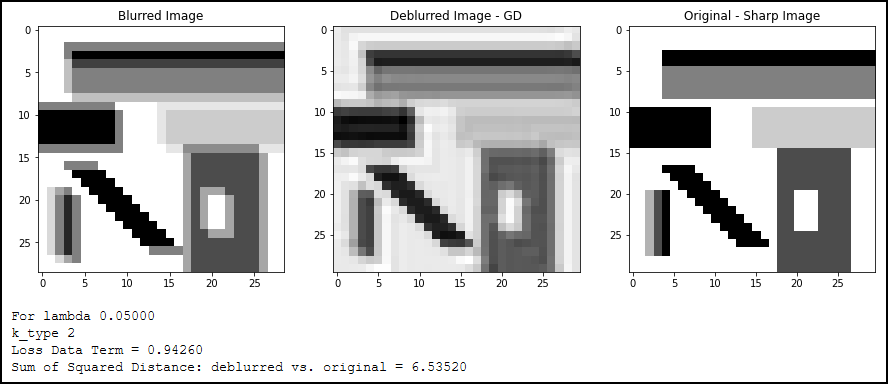
\includegraphics[scale=0.31]{GD_GP_0500.png}
					\caption{GD - \textit{Gaussian Prior}, $\lambda = 0.05$}
					\label{fig:GD_GP05}
				\end{subfigure}
				\begin{subfigure}[b]{0.45\textwidth}
					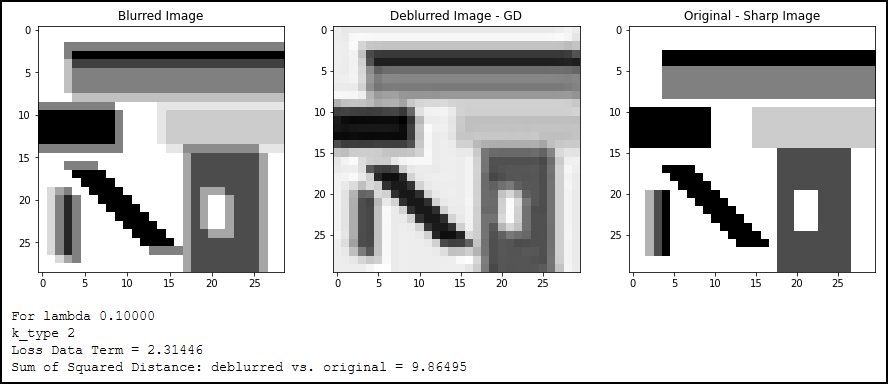
\includegraphics[scale=0.31]{GD_GP_1000.png}
					\caption{GD - \textit{Gaussian Prior}, $\lambda = 0.1$}
					\label{fig:GD_GP1}
				\end{subfigure}
			\end{figure}
			\subsubsection*{Anisotropic Total Variation}
			\begin{figure}[H] \renewcommand\thesubfigure{GD.ATV.\arabic{subfigure}}
				\centering
				\begin{subfigure}[b]{0.45\textwidth}
					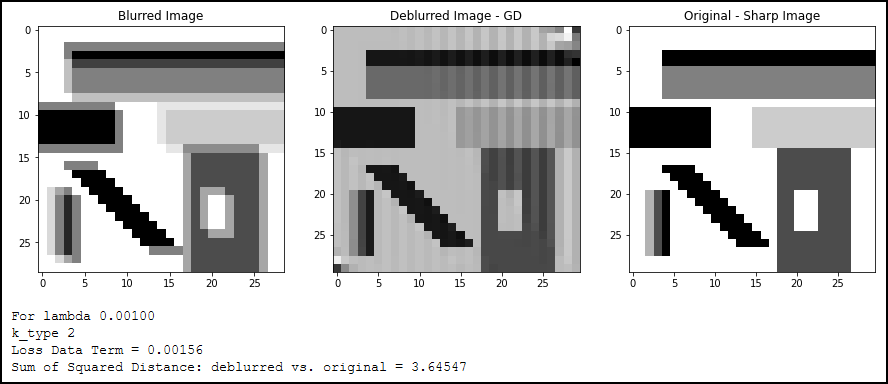
\includegraphics[scale=0.31]{GD_ATV_0010.png}
					\caption{GD - \textit{Anisotropic TV}, $\lambda = 0.001$}
					\label{fig:GD_ATV001}
				\end{subfigure}
				\begin{subfigure}[b]{0.45\textwidth}
					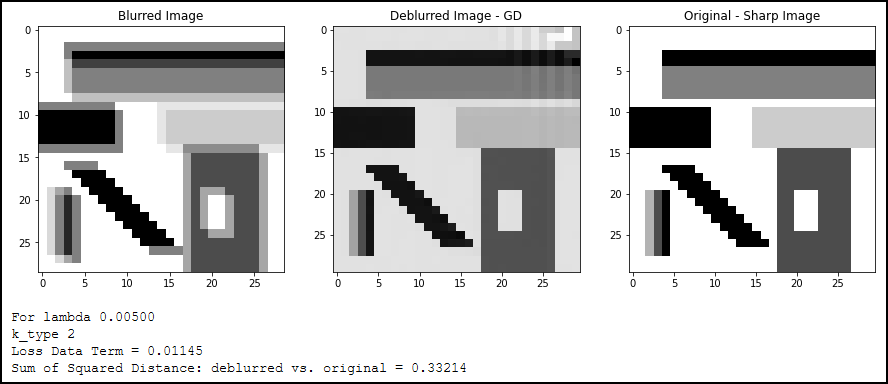
\includegraphics[scale=0.31]{GD_ATV_0050.png}
					\caption{GD - \textit{Anisotropic TV}, $\lambda = 0.005$}
					\label{fig:GD_ATV005}
				\end{subfigure}
				\\
				\centering
				\begin{subfigure}[b]{0.45\textwidth}
					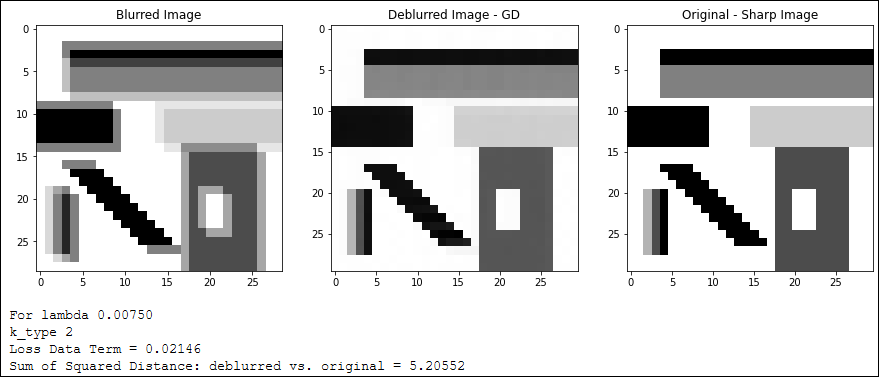
\includegraphics[scale=0.31]{GD_ATV_0075.png}
					\caption{GD - \textit{Anisotropic TV}, $\lambda = 0.0075$}
					\label{fig:GD_ATV0075}
				\end{subfigure}
				\begin{subfigure}[b]{0.45\textwidth}
					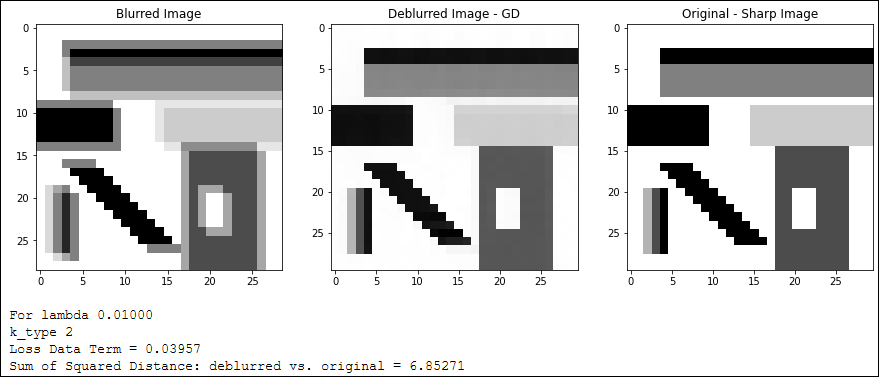
\includegraphics[scale=0.31]{GD_ATV_0100.png}
					\caption{GD - \textit{Anisotropic TV}, $\lambda = 0.01$}
					\label{fig:GD_ATV01}
				\end{subfigure}
				\\
				\centering
				\begin{subfigure}[b]{0.45\textwidth}
					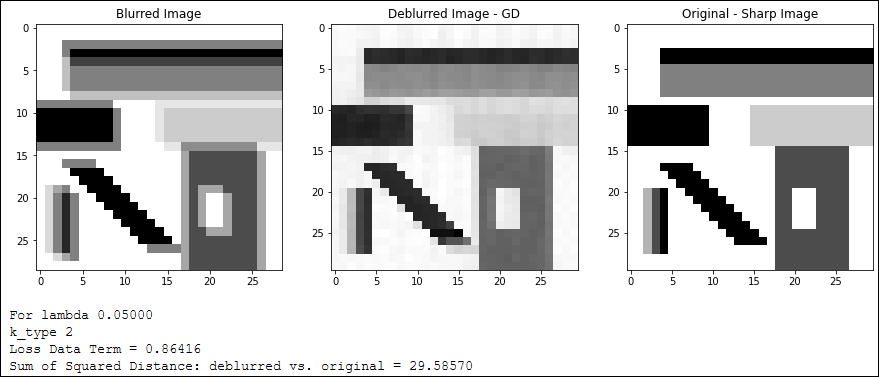
\includegraphics[scale=0.31]{GD_ATV_0500.png}
					\caption{GD - \textit{Anisotropic TV}, $\lambda = 0.05$}
					\label{fig:GD_ATV05}
				\end{subfigure}
				\begin{subfigure}[b]{0.45\textwidth}
					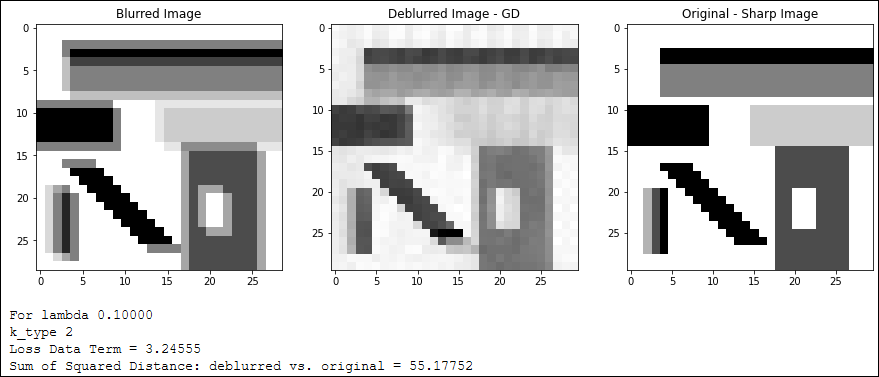
\includegraphics[scale=0.31]{GD_ATV_1000.png}
					\caption{GD - \textit{Anisotropic TV}, $\lambda = 0.1$}
					\label{fig:GD_ATV1}
				\end{subfigure}
			\end{figure}
		\closesection
	\closesection
	\newpage
	
	\section{Linearization + Gauss-Seidel}
	\startsection
	\closesection
	
	\section{Linearization + SOR}
	\startsection
	\closesection
	
	\section{Other Questions}
	\startsection
		\subsection{Effect of the $\lambda$ value}
		\startsubsection
		\closesection
		\subsection{Sum of Squared Distances}
		\startsubsection
		\closesection
	\closesection
\end{document}